\subsection{Triggering and data collection}
While in full operation for the 2012, 8~TeV run, the LHC delivered a bunch crossing in \textsc{atlas}' interaction point every 50~ns. Reading out the whole detector produces 1.6~MB of information, which, if the detector were read out completely with every crossing, would produce a data rate of 34~TB/s.\footnote{For perspective, that is approximately equal to the estimated global IP traffic rate in 2015, according to \cite{wolframip}.} However, since only a fraction of these collisions produce interesting physics events, we can reduce the data rate to less prohibitive levels simply by not recording data from collision that do not produce interesting events. To accomplish this, we need a system that examines events in the detector as they occur, and trigger recording whenever it sees an interesting event. In \textsc{atlas}, this trigger system has three levels, which are described in detail in \cite{detectorpaper}. 

The level--1 trigger genuinely does examine events as they occur in the detector. To do so, it runs on specialised hardware built in to the detectors, and as a result, it only has access to the raw information from the detectors to which it is attached. This means, for example, that track reconstruction is not available when the level--1 trigger deicdes whether or not to record an event. The next trigger level, level--2, is run on the full set of information on an event, on those events which pass the level--1 filter. The final trigger level works with fully reconstructed events and derived physical observables. This requres more time and processing power than is available at the previous levels, but it also identifies interesting events with the same quality of information as will be used in the subsequent analysis. All three triggers in combination cuts the final event rate to 300 events per second, with a peak rate of 600 events.

For this thesis, we shall use data taken during the 8~TeV run in 2012. The amount of data taken at any given time depends on the condiitions of the beam, which can be summarised in the instantaneous luminosity, and the conditions of the detector, which may only capture a fraction of the events produced at any given time. Figure~\ref{intlumi} gives the distribution of integrated and captured luminosity over the course of the year.

\begin{figure}[htp]
\begin{minipage}[b]{.69\textwidth}
\hspace{-1em}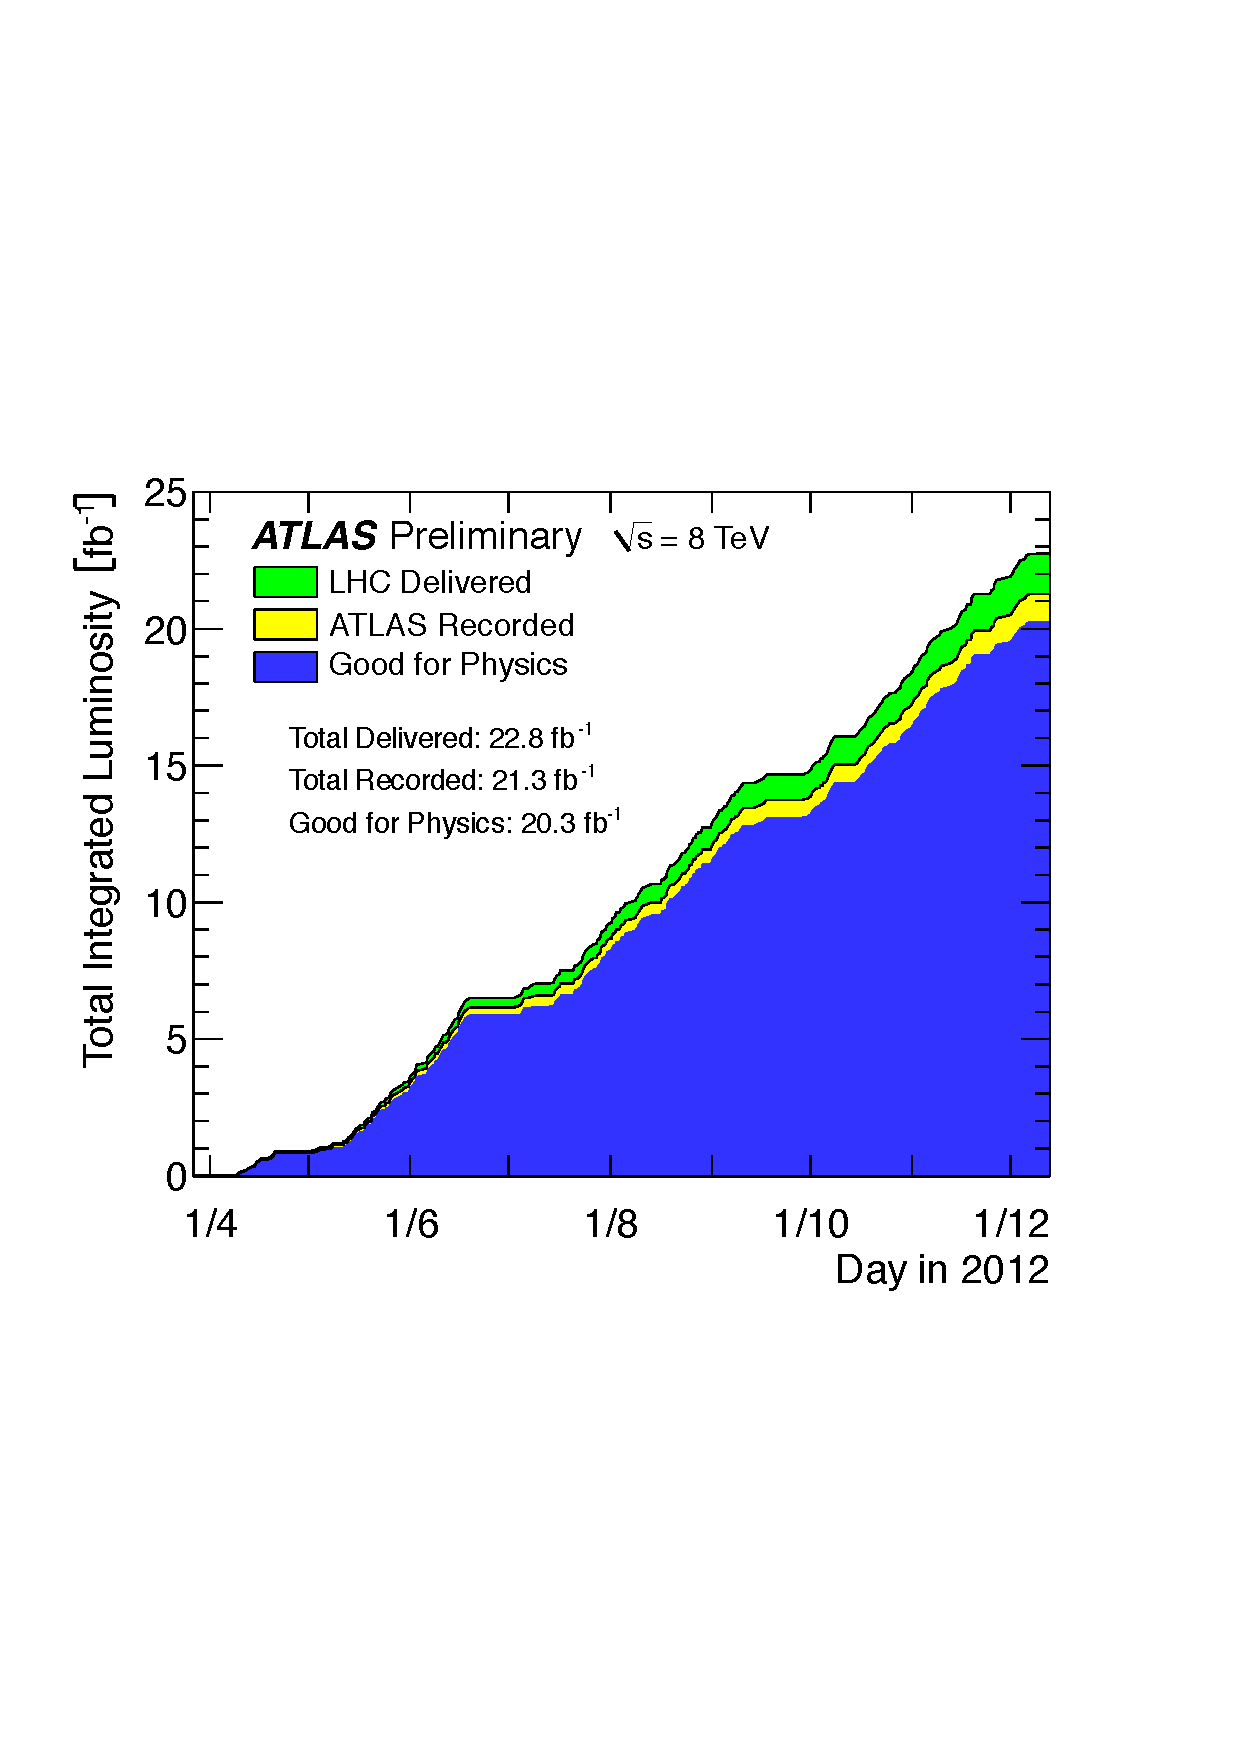
\includegraphics[width=\textwidth]{figures/intlumi}
\end{minipage}\hfill\begin{minipage}[b]{.3\textwidth}
\caption{A plot showing the integrated luminosity delivered by the LHC (green), recorded by ATLAS (yellow), and fulfilling data quality criteria (blue), over the course of the 8 TeV run in 2012 \cite{publiclumi}.
\label{intlumi}}
\end{minipage}
\end{figure}

Unfortunately, the triggers that \atlas{} implements do not guarantee that the event rate remains within the technical limitations of the readout system. to stay within those limits, \atlas{} removes a fraction of the events that did pass the triggers, when they originate from a trigger that produces more events than it is considered worth keeping.\footnote{Explaining how it is decided whether data is worth keeping would veer into a discussion of \atlas{} internal politics, which is a topic beyond the scope of this thesis.} The diphoton channel is important to the search for the Higgs boson, however, so the triggers that produce diphotons events are not prescaled in this fashion.


\chapter{Data preparation}

For the present analysis, we will use events that passed the \texttt{2g40\_loose} level--1 trigger, which requires that the EM calorimeter reports two hits with at least 40~GeV of transverse energy that pass the loose selection criteria, described in the previous chapter.

The datasets have been retrieved in the \texttt{NTUP\_PHOTON} format, which is streamlined to contain information relevant to photon analyses, and easily readable by \textsc{root}. The dataset used contains events corresponding to 18.301~fb$^{-1}$ of integrated luminosity.

On each of the prospective photons in this dataset, we impose a series of selection criteria:

\begin{itemize}
\item \textbf{otx and phoCloan cut:} Object quality cuts, which cut out events too close to non-functioning or noisy detector elements, and events taken while the detector was in a non-optimal state.
\item \textbf{ID cut:} Objects that did not pass photon identification, or do not satisfy the loose selection criteria after reconstruction, are eliminated.
\item \textbf{kinematics cut:} Ensures that objects do not have $|\eta|$ greater than 2.37, which is the forward limit of the first layer of the EM calorimeter, or in the range between 1.37 and 1.52, which is the transition region between the barrel and endcap calorimeters. Also ensures $E_T$ greater than 50~GeV, which clears the turn--on curve of the \texttt{2g40\_loose} trigger.
\item \textbf{N\_events cut:} Ensures that each event has at least two photons that pass the above criteria.
\item \textbf{PV cut:} Ensures that the photon pair selected for analysis have the same primary vertex, and that that vertex has at least three tracks associated with it.

\end{itemize}

The number of objects remaining at each step of the cut procedure is plotted in figure~\ref{cutflow}

\begin{figure}[htp]
\begin{minipage}[b]{.69\textwidth}
\hspace{-1em}%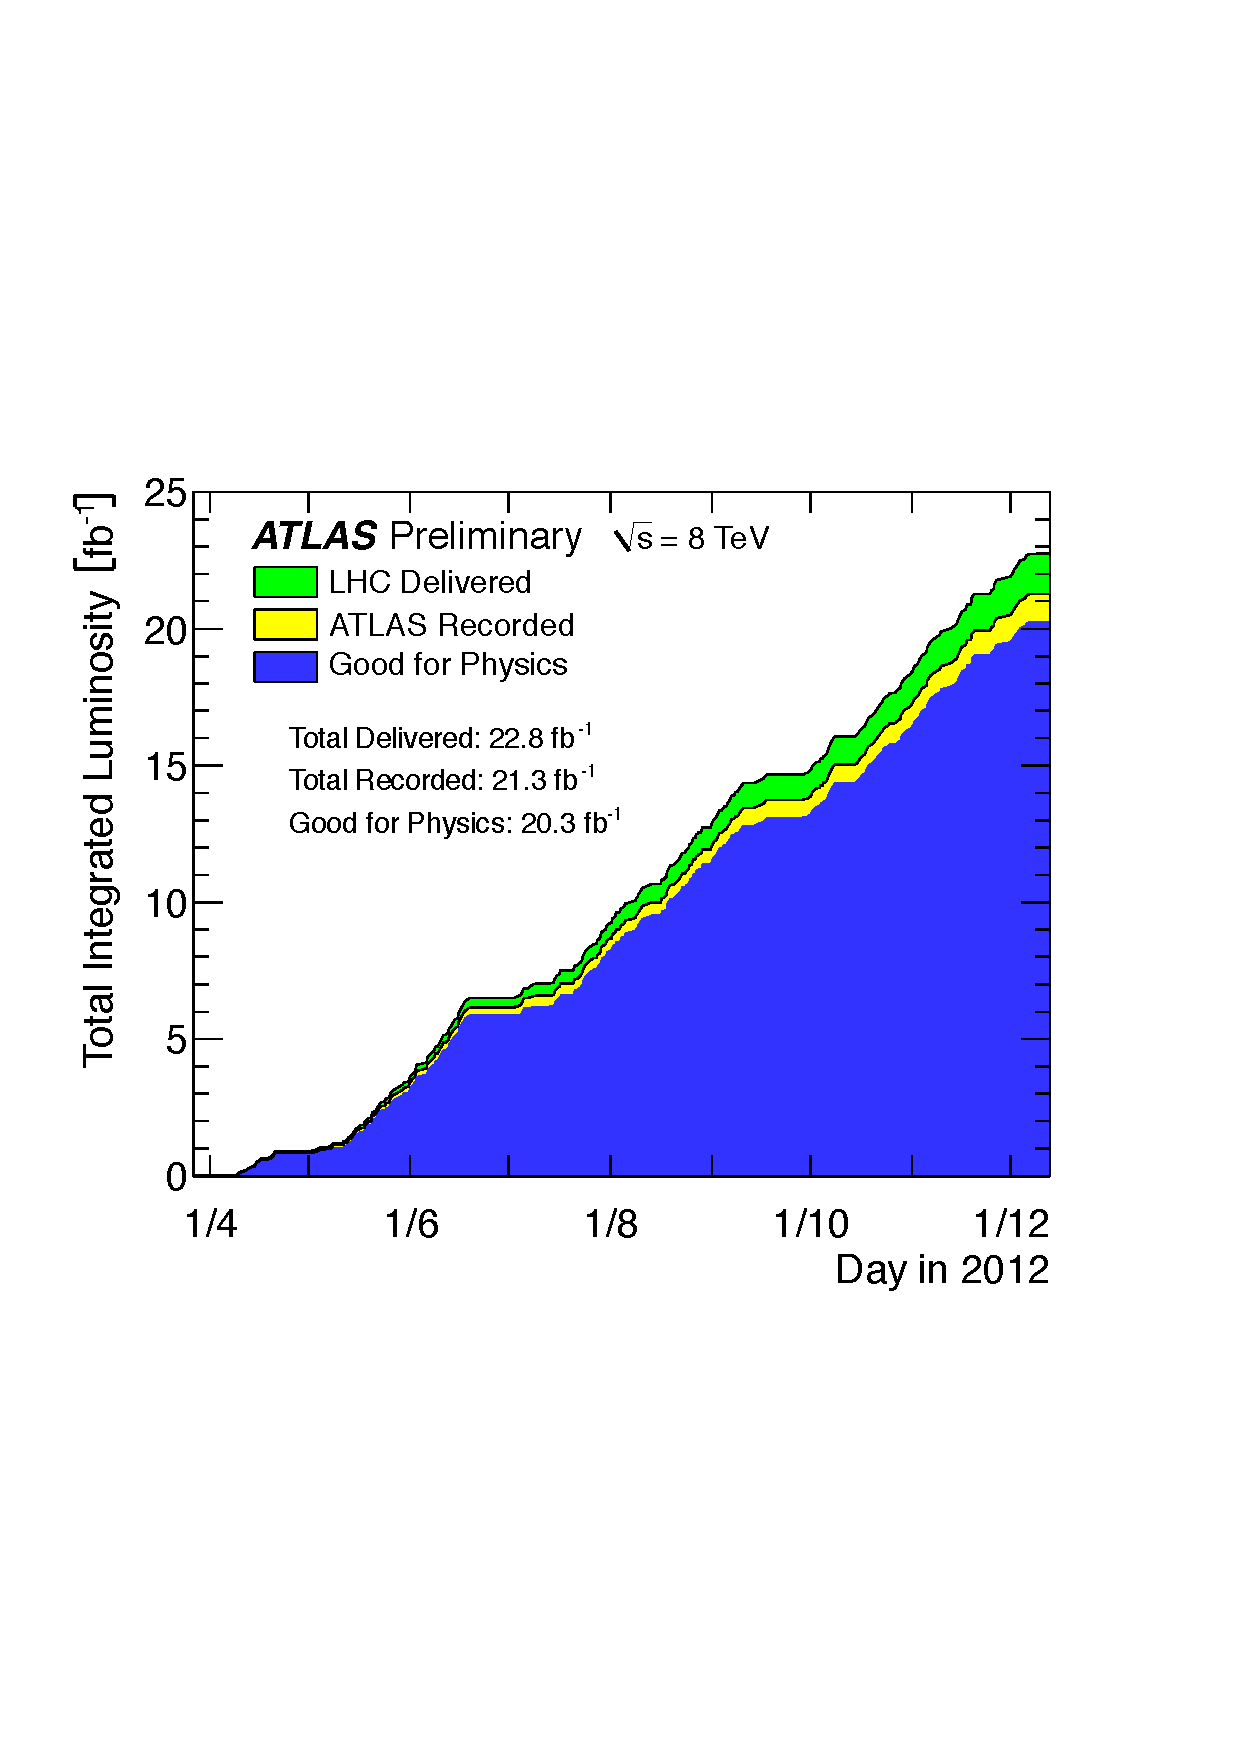
\includegraphics[width=\textwidth]{figures/intlumi}
\centering (a very impressive plot.)
\end{minipage}\hfill\begin{minipage}[b]{.3\textwidth}
\caption{A cutflow diagram, showing how many objects remain in the dataset after each of the selection criteria are imposed. The final number of photons is (something I sould be able to dig up somewhere).
\label{cutflow}}
\end{minipage}
\end{figure}

\section{Background filtering}
Then, knowing that background events have snuck their way into our data sample, we venture into some data-driven background subtraction methods. These will, if and when they work, be:

\subsection{The ABCD method}
Our old friend. And:

\subsection{The S-frame method}
Or however the hell you're supposed to render that. If it works.

Incidentally, the presence of pileup events probably means that we should run the MC events through this machinery as well. Even if we aren't filtering out the same things, we are filtering out \textit{some} of the same things, albeit, presumably, imperfectly(, natch). There are also things that aren't there, that we're not filtering out imperfectly, and so won't be there. But it's an imperfect world.

This should leave us with the sample of events that we will use to estimate $\Lambda$.
